\documentclass[a4paper,11pt]{article}
\usepackage{amsmath} 
\usepackage{amsfonts}
\usepackage{graphicx}
\usepackage{algorithm,algorithmic}
\usepackage{url}
\usepackage{color}
\usepackage{tikz}
\usepackage{multirow}
\usepackage{verbatim}
\usepackage{hyperref}
\usepackage{float}
\usepackage{geometry}
\usepackage{indentfirst}
\usepackage{amssymb}

\usepackage{listings}
\usepackage{makeidx}

\usepackage{times}
\usepackage{graphicx}

\usepackage{longtable}




\usetikzlibrary{shapes,arrows}
\geometry{left=3.17cm,right=3.17cm,top=2.54cm,bottom=2.54cm}
%\begin{comment}
\pagestyle{empty}
%\end{comment}
\begin{document}
\begin{center}
{\large The secondary emission model used in OPAL} \\
Chuan Wang, Andreas Adelmann \\
\today\\
\end{center}
\section{Introduction}
The secondary emission module in OPAL (in a test program at present) is based on the models developed at Lawrence Berkeley National Laboratory \cite{SE}.  For the electron-induced secondary electron routines, the total yield is returned, as well as the dimensionless components of normalized velocity $\beta$. The velocity components are returned as arrays of length 10, corresponding to the model parameters. Presently, these routines contain material models for copper and stainless steel only.\\

We choose this secondary model because it is mathematically self-consistent; by this we mean that, if we define one incident electron and the followed secondary emission as an event, the event generator is constructed so that (1) when averaging over an infinite number of secondary-emission events, the reconstructed secondary emission yield $\delta$ and its energy spectrum $ d\delta/dE$ are guaranteed to agree with  the corresponding input quantities; (2) the energy integral of $ d\delta/dE$ is guaranteed to equal $\delta$; (3) the energy of any given emitted electron is guaranteed not to exceed the primary energy; and (4) the aggregate energy of the electrons emitted in any multi-electron event is also guaranteed not to exceed the primary energy. The basic computational procedure is as follows:\\
\begin{figure}[H]
\begin{center}
%\usepackage[latin1]{inputenc}
%\usepackage{tikz}
%\usetikzlibrary{shapes,arrows}

%<
%\usepackage{verbatim}
%\usepackage[active,tightpage]{preview}
%\PreviewEnvironment{tikzpicture}
%\setlength\PreviewBorder{5pt}%
%



% Define block styles
\tikzstyle{decision} = [draw,diamond, fill=blue!20, 
    text width=4.5em, text badly centered, node distance=2.2cm, inner sep=0pt]
\tikzstyle{block} = [draw,rectangle, fill=blue!20, 
    text width=7.5em, text badly centered, inner sep=3pt, rounded corners, minimum height=4em]
\tikzstyle{line} = [draw, -latex']
\tikzstyle{cloud} = [draw, \ellipse,fill=red!20, node distance=2.2cm,
    minimum height=2em]
\tikzstyle{every node}=[font=\small]
\scalebox{0.75}{
\begin{tikzpicture}[node distance = 2.2cm, auto, every node/.style={anchor=base,font=\small}]
    % Place nodes
    \node [block] (incident) {Incident $E_0$, $\theta_0$};
   % \node [cloud, left of=incident] (expert) {expert};
   % \node [cloud, right of=incident] (system) {system};
    \node [block, below of=incident, node distance=2.2cm] (yield) {Compute $\delta_e(E_0,\theta_0)$, $\delta_r(E_0,\theta_0)$, $\delta_{ts}(E_0,\theta_0)$};
    \node [block, below of=yield, node distance=2.2cm] (probability) {Compute $P_n, n=0,1,...,M$};
    \node [block, below of=probability, node distance=2.5cm] (secondaryNum) {Random integer $n$ with probability distribution $\{P_n\}$};
    \node [decision, right of=incident, node distance=3.5cm] (decide) {$n=0$?};
    \node [block, right of=decide, node distance=3.5cm] (zero) {Delete the incident electron};
    \node [decision, below of=decide, node distance=3.0cm] (decide1) {$n=1$?};
    \node [block, right of=decide1, node distance=3.5cm] (one) {Emitted energy $E\in[0,E_0]$ with PDF $f_{1,e}+f_{1,r}+f_{1,ts}$ };	\node [block, below of=decide1, node distance=3.5cm] (ts) {Emitted energy $E_k\in[0,E_0]$, $k=1,...,n$ with PDF $f_{n,ts}$ };
    \node [block, below of=one, node distance=3.5cm] (angle) {Generate $\theta_k\in[0,\pi/2]$, with PDF $cos^{\alpha}$; and $\phi_k\in[0,2\pi]$, $k=1,...,n$. Calc momenta accordingly. };
    % Draw edges
    \path [line] (incident) -- (yield);
    \path [line] (yield) -- (probability);
    \path [line] (probability) --  (secondaryNum);		
   % \path [line] (probability) -- (secondaryNum);
   % \path [line] (decide) -- node [near start] {$No$} (secondaryNum);
    \draw[->] (secondaryNum) -| +(1.8,3) |- (decide);
    %\path [line] (decide) -- node [near start,above] {yes} (zero);
    \draw[->] (decide) -- node [midway,above=2pt] {yes} (zero);	
    \path [line] (decide) -- node [midway,right=2pt] {no} (decide1);
    \path [line] (decide1) -- node [midway,above=2pt] {yes} (one);
    \path [line] (decide1) -- node [midway,right=2pt] {no} (ts);
    \path [line] (ts) -- (angle);

    \path [line] (one) -- (angle);
    \path [line] (zero) -- +(0,1.5)-| node [near start,above=2pt] {Next event} (incident);
    \path [line] (angle) -- +(0,-2.)--  node [midway,above=2pt] {Next event} (-2,-8.65) |- (incident) ;
 %\path [line] (secondaryNum) -|- (decide);
  %  \path [line] (decide) -- node {no}(stop);
   % \path [line,dashed] (expert) -- (incident);
  %  \path [line,dashed] (system) -- (incident);
   % \path [line,dashed] (system) |- (probability);
\end{tikzpicture}
}

\end{center}
\caption{  Basic computational procedure of secondary emission model .\label{fig:P-B}}
\end{figure}
There is another assumption to reduce the complexity of the model, i.e., the backscattered and rediffused electrons only exist when the emitted electron number $n = 1$.

\section{Computation of SEY}
\subsection {SEY of backscattered electrons}
The SEY of backscattered electrons $\delta_e(E_0,\theta_0)$ with incident energy $E_0$ and  incidental angle ($\theta_0$) might be given by 
\begin{equation*}
\delta_e(E_0,\theta_0) = \delta_e(E_0,0)[1+e_1(1-\cos^{e_2}{\theta_0})]
\end{equation*}
where,
\begin{equation*}
\delta_e(E_0,0) = P_{1,e}(\infty)+[\hat{P}_{1,e}-P_{1,e}(\infty)]e^{-(\left|E_0-\hat{E}_e\right|/W)^P/P}
\end{equation*}
Here, $e_1$, $e_2$, $ P_{1,e}(\infty)$, $\hat{P}_{1,e}$, $\hat{E}_e$, $W$ and $P$ are material related parameters to fit the experimental data.
\subsection {SEY of rediffused electrons}
The SEY of rediffused electrons $\delta_r(E_0,\theta_0)$ with incident energy $E_0$ and  incidental angle ($\theta_0$) might be given by 
\begin{equation*}
\delta_r(E_0,\theta_0) =  \delta_r(E_0,0)[1+r_1(1-\cos^{r_2}{\theta_0})]
\end{equation*}
where,
\begin{equation*}
\delta_r(E_0,0) = P_{1,r}(\infty)[1-e^{-(E_0-E_r)^r}]
\end{equation*}
Here, $r_1$, $r_2$, $ P_{1,r}(\infty)$, $E_r$ and $r$ are material related parameters to fit the experimental data.
\subsection {SEY of true secondary electrons}
The SEY of true secondary electrons $\delta_r(E_0,\theta_0)$ with incident energy $E_0$ and incidental angle ($\theta_0$) might be given by 
\begin{equation*}
\delta_{ts}(E_0,\theta_0) = \hat{\delta}(\theta_0)D[E_0/\hat{E}(\theta_0)]
\end{equation*}
where, 
\begin{equation*}
\hat{\delta}(\theta_0) = \hat{\delta}_{ts}[1+t_1(1-\cos^{t_2}{\theta_0})]
\end{equation*}
\begin{equation*}
\hat{E}(\theta_0) = \hat{E}_{ts}[1+t_3(1-\cos^{t_4}{\theta_0})]
\end{equation*}
\begin{equation*}
D(x) = \frac{sx}{s-1+x^s}
\end{equation*}
where, $ \hat{\delta}_{ts} $, $ \hat{E}_{ts} $, $t_1$, $t_2$, $t_3$, $t_4$ and $s$ are material related parameters to fit the experimental data.
\section{Computation of emission probability $\{P_n\}$}
To avoid the situation in the definition of probability per incident electron that $P_1$ can exceed unity and $P_0$ can become negative even if $\delta_e$ and $\delta_r$ are constrained to satisfy $\delta_e+\delta_r \leq 1$, we first calculate the probability per penetrated electron $\{P'_n\}$. Here we choose for $\{P'_n\}$ the binomial distribution:
\begin{equation*}
P'_{n,ts} = \binom{M}{n}p^n(1-p)^{M-n}, 0 \leq n \leq M,
\end{equation*}
where $p = \langle n \rangle /M = \delta'_{ts}/M$, $\delta'_{ts} = \frac{\delta_{ts}}{1 - \delta_{e} - \delta_{r}}$. And $M$ must be chosen $> \delta'_{ts}$ to insure that $p$ must be $< 1$. In our practical case, we choose $M = 10$. Then the overall emission probabilities will be
\begin{equation*}
P_0 = (1 - \delta_e - \delta_r)P'_{0,ts},
\end{equation*}
\begin{equation*}
P_1 = (1 - \delta_e - \delta_r)P'_{1,ts} + \delta_e + \delta_r,
\end{equation*}
\begin{equation*}
P_n = (1 - \delta_e - \delta_r)P'_{n,ts}, n \geq 2,
\end{equation*}
Here, we should point out that $\delta_e$, $\delta_r$, $\delta_{ts}$ are short form of $\delta_e(E_0,\theta_0)$, $\delta_r(E_0,\theta_0)$, $\delta_{ts}(E_0,\theta_0)$ respectively.
\section{Computation of emission number, energy, angle distribution and momenta}
\subsection{Computation of emission number}
We get the emitted secondary electron number by using a Monte Carlo procedure. We first generate random number $r_u \in [0,1]$ with distribution $\{P_n\}$ by using acceptance-rejection method and then we get the emitted secondary number $n$ by
\begin{equation*}
n = \lfloor r_u \times M \rfloor
\end{equation*} 
\subsection{Computation of emitted energy}
If the emitted secondary electron number $n = 0$, then we just mark the incident electron for further deletion.\\

If the emitted secondary electron number $n = 1$, the emitted energy $E \in [0,E_0]$ has the following distribution density:
\begin{equation*}
\rho(E) = a_e\rho_e(E) + a_r\rho_r(E) + a_{ts}\rho_{ts}(E),
\end{equation*}
where $\rho^,$s are probability densities with unit normalization, defined by
\begin{equation*}
\rho_e(E) = f_{1,e}(E)/\delta_e(E_0),
\end{equation*}
\begin{equation*}
\rho_r(E) = f_{1,r}(E)/\delta_r(E_0),
\end{equation*}
\begin{equation*}
\rho_{ts}(E) = f_{1,ts}(E)/P_{1,ts}(E_0),
\end{equation*}
The weights $a_i^,$s satisfy $a_i>1$ and $a_e + a_r + a_{ts} = 1$. These weights are given by
\begin{equation*}
a_{e}(E) = \delta_e(E_0)/\delta_1(E_0),
\end{equation*}
\begin{equation*}
a_{r}(E) = \delta_r(E_0)/\delta_1(E_0),
\end{equation*}
\begin{equation*}
a_{ts}(E) = P_{1,ts}(E_0)/\delta_1(E_0),
\end{equation*}
where $\delta_1(E_0) = \delta_e(E_0) + \delta_r(E_0) + P_{1,ts}(E_0)$. The algorithm to generate E is the following:
\begin{algorithm}[H]
   \caption{Algorithm to generate E when n = 1} \label{alg:ge_algo}
   \begin{algorithmic}[1]
     \STATE Generate a uniformly distributed random number $u \in [0,1]$.
     \IF{$0 \leq u < a_e$}
     \STATE Generate $E$ with PDF $\rho_e(E)$, i.e., $E = E_0 - \sigma_e\left| g \right|$, $g$ is a standard normal random number.
     \ENDIF
     \IF{$a_e \leq u < a_e + a_r$}
     \STATE Generate $E$ with PDF $\rho_r(E)$, i.e., $E = E_0u_1^{1/(1+q)}$, $u_1 \in [0,1]$ is another uniformly distributed random number.
     \ENDIF
     \IF{$a_e + a_r \leq u < 1$}
     \STATE Generate $E$ with PDF $\rho_{ts}(E)$, i.e., $E = \epsilon_1P^{-1}(p_1,u_2P_0)$, $u_2 \in [0,1]$ is another uniformly distributed random number, $P(p,x)$ is the normalized in complete gamma function, $P_0 = P(p_1,E_0/\epsilon_1)$, $P^{-1}(p_1,x)$ is the functional inverse (in x) of $P(p,x)$.
     \ENDIF
   \end{algorithmic}
 \end{algorithm}
Here $\sigma_e$, $q$, $p_1$ and $\epsilon_1$ are all material related parameters to fit the experimental data.\\

If the emitted secondary electron number $n \geq 2$, the emitted energy $E_k \in [0,E_0], k = 1,...n$ has the following probability density subject to $x_k \geq 0$:
\begin{equation*}
\frac{dN}{d^n\mathbf{x}} \propto \theta(x_0 - x_1 - \ldots - x_n)\prod_{k=1}^nx_k^{p-1}e^{-x_k} 
\end{equation*}
where $\mathbf{x} = (x_1,x_2,\ldots,x_n)$, $x_k = E_k/\epsilon_n, k = 1,2,\ldots,n$. Specially, $x_0 = E_0/\epsilon_n$. Here $p = p_n$ and $\epsilon_n$ are material related parameters to fit the experimental data. To obtain the emitted energy serial $\{E_k\}$ accordingly by using Monte Carlo method, a new vector $\mathbf{y}$ has to be defined by $y_k = x_k^2$. Using n-dimensional spherical coordinates for $\mathbf{y}$, we get
\begin{equation*}
\left. \begin{array}{c}
y_1 = y\cos{\theta_1},\\
y_2 = y\sin{\theta_1}\cos{\theta_2},\\
y_3 = y\sin{\theta_1}\sin{\theta_2}\cos{\theta_3},\\
\vdots\\
y_{n-1} = y\sin{\theta_1}\sin{\theta_2}\ldots\cos{\theta_{n-1}},\\
y_{n} = y\sin{\theta_1}\sin{\theta_2}\ldots\sin{\theta_{n-1}},\\
\end{array} \right\}
\end{equation*}
Where $\theta_k$ are stochastically generated by 
\begin{equation*}
\theta_k = \arcsin{\sqrt{\hat{\beta}^{-1}(u_k,\mu,\nu)}}
\end{equation*}
The amplitude $y$ is given by
\begin{equation*}
y = \sqrt{P^{-1}(np,uP_0)}
\end{equation*}
Here, $u_k \in [0,1]$ is the $k th$ uniformly distributed random number, $\mu = p(n-k)$, $\nu = p$, $p = p_n$, $\hat{\beta}^{-1}$ is the functional inverse (in x) of incomplete beta function, $P^{-1}(np,x)$ is the functional inverse (in x) of incomplete gamma function $P(np,x)$, $u \in [0,1]$ is a uniformly distributed random number and $P_0 = P(np,x_0)$.\\

The computational algorithm for generating energy serial $\{E_k\}$ could be summarized as the following:
\begin{algorithm}[H]
   \caption{Algorithm to generate $\{E_k\}$ when $n \geq 2$} \label{alg:ge2_algo}
   \begin{algorithmic}[1]
     \STATE Compute $x_0 = E_0/ \epsilon_n$ and $P_0 = P(np,x_0)$.
     \STATE Generate $n-1$ uniformly distributed random numbers $u_k \in [0,1] (k = 1,\ldots,n-1)$ and compute $\theta_k$.
     \STATE Generate one more uniformly distributed random numbers $u \in [0,1]$ and compute $y$.
     \STATE Compute vector $\mathbf{y}$.
     \STATE Compute energies using $E_k = \epsilon_nx_k = \epsilon_ny_k^2$ for $k = 1,\ldots,n$
   \end{algorithmic}
 \end{algorithm}
Here $p = p_n$ and $\epsilon_n$ are material related parameters to fit the experimental data as previous situation. 
\subsection{Computation of emitted angles}
The emitted angles can be easily obtained by using Monte Carlo method. First generate $n$ independent polar angles $\theta_k \in [0,\pi/2]$ ($\theta_k$ here is not the same with the variable in the previous section) with probability density $\cos^{\alpha}{\theta}$. The second, generate $n$ independent azimuthal angles $\phi_k \in [0,2\pi]$. The above angles are relative to the local coordinate system that is centered at collision point and whose $z$ axis is along the inward normal to the chamber surface.
\subsection{Computation of momenta}  
We can easily get the normalized non unit velocity $\beta$ and momenta $\beta\gamma$ since the kinetic energy is obtained and as the emitted angles are known the momenta in various coordinate systems could be obtained accordingly.
\section{The math needed in this secondary emission model}
\subsection{Special functions}
GNU scientific library (GSL) has already been included in OPAL. But unfortunately there are neither inverse incomplete beta function nor inverse incomplete beta function in GSL. So we choose the algorithms in reference \cite{NR} to obtain the numerical evaluation of inverse incomplete beta function and inverse incomplete beta function.
\subsection{Random number with specified distributions}
Here, we use the random generator in our IPPL library to generate the uniformly distributed random number which are needed when we generate random number with specified distributions. Most of the specified distributions in the previous sections are calculated by using inverse PDF of uniformly distributed variables.\\

The standard normal distributed random number is generated by using a so called polar form of the Box-Muller transformation. The detailed algorithm can be found in reference \cite{GR}.\\

And a so called acceptance-rejection method is used to generate random number with distribution $\{P_n\}$ when we calculate the number of emitted secondary electrons.
\section{Code to code comparison}
In order to validate the secondary module to be implemented in OPAL, we have conducted a code to code comparison with TxPhysics library \cite{TP}. We have initialized a large number of incident events (10000) with the same energy (300eV) and the same incident angle (normal to the surface). Then we marked and plot the emitted secondary energy. The result from the secondary module in both OPAL and TxPhysics is shown in Figure \ref{fig:cc}. It is obvious that the results are statistically matched. 

\begin{figure}[H]
\begin{center}
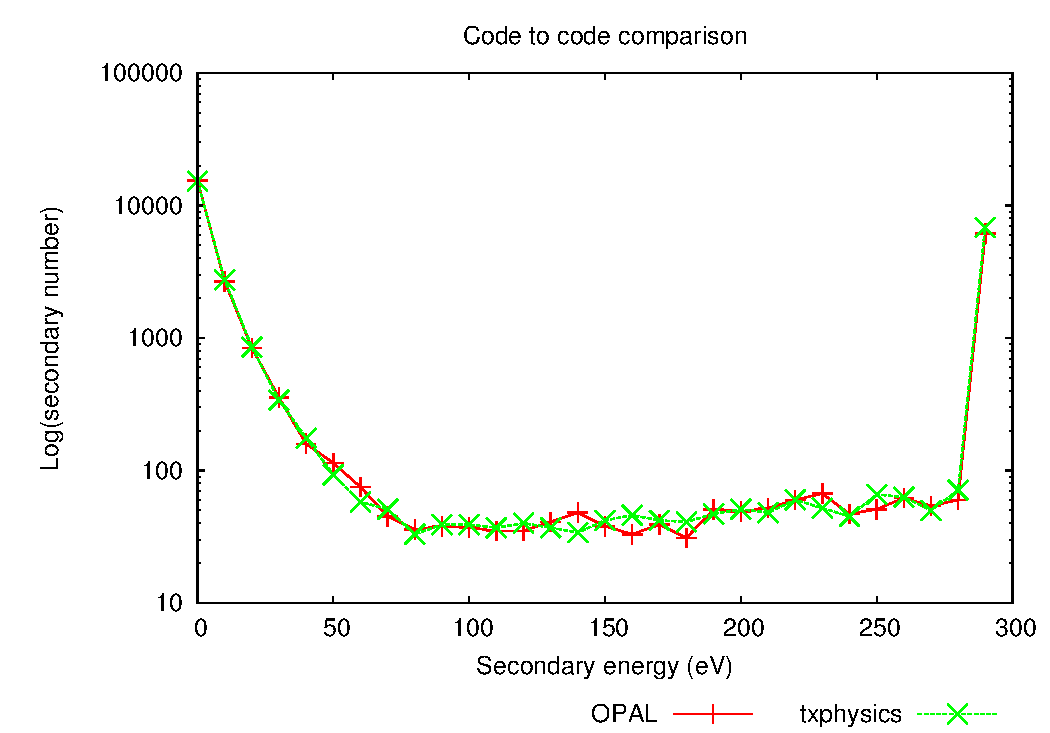
\includegraphics[width=1\textwidth]{code_comparison.pdf}
\end{center}
\caption{Secondary energy comparison between OPAL and TxPhysics\label{fig:cc}}
\end{figure}
\begin{thebibliography}{99}
\bibitem{SE}  M. A. Furman and M. Pivi, Phys. Rev. ST Accel. Beams 5, 124404 (2002)
\bibitem{NR} W. H. Press, S. A. Teukolsky, W. T. Vetterling and B. P. Flannery, NUMERICAL RECIPES-The Art of Scientific Computing, 3rd ed., Cambridge Press, Cambridge, (2007), pp. 259-273
\bibitem{GR} Available Online on: \href{http://www.taygeta.com/random/gaussian.html}{http://www.taygeta.com/random/gaussian.html}
\bibitem{TP} Txphysics library: Advanced physics for accelerator simulations. Available Online on: \href{http://www.txcorp.com/products/TxPhysics/}{http://www.txcorp.com/products/TxPhysics/}
\end{thebibliography}
 
\end{document}